\section{Computational model}

        Il modello migliore è stato ottenuto dopo una prima fase di \textit{data preparation}, ed una successiva fase di \textit{hyper-parameter tuning}.

        \subsection{Data preparation}
        
                \subsubsection{Data splitting}
                
                        Il \textit{dataset} è stato diviso in due sezioni differenti:
                        \begin{itemize}
                                \item \textit{training set}: contiene 80\% dell'intero dataset originale (6400 records)
                                \item \textit{test set}: contiene il restante 20\% del dataset originale (1600 records)
                        \end{itemize}
                
                \subsubsection{Bad values management}
                
                        Il \textit{dataset} originale contiene dati mancanti in corrispondenza di alcune delle \textit{features}, per questo motivo, i valori relativi a tali campi sono stati sostituiti con il valore medio della \textit{feature} all'interno del \textit{dataset}.
                        \bigbreak
                        
                        Per l'individuazione degli \textit{outlier} sono stati analizzati i risultati derivanti da tre metodi:
                        \begin{itemize}
                            \item \textit{z-score}
                            \item \textit{modified z-score}
                            \item \textit{inter-quartile range}
                        \end{itemize}
                        
                        \textbf{TODO - descrivere in formule gli approcci dei 3 metodi}
                        
                        Per non ridurre la numerosità del \textit{training set} si è scelto di sostituire (e non eliminare) gli \textit{outliers} con la mediana relativa ad una determinata \textit{feature}. Si è ritenuto opportuno utilizzare la mediana in quanto è una misura più robusta per la rappresentazione della dispersione di valori rispetto alla media essendo meno soggetta alla presenza di \textit{outliers}.                        
                
                \subsubsection{Data normalization}
                
                \subsubsection{Feature selection}
                
                        In questa fase sono state selezionate le \textit{features} più significative al fine di ridurre i costi di training e migliorare la capacità di generalizzazione del classificatore.
                        
                        \begin{figure}[!h]
                            \centering
                            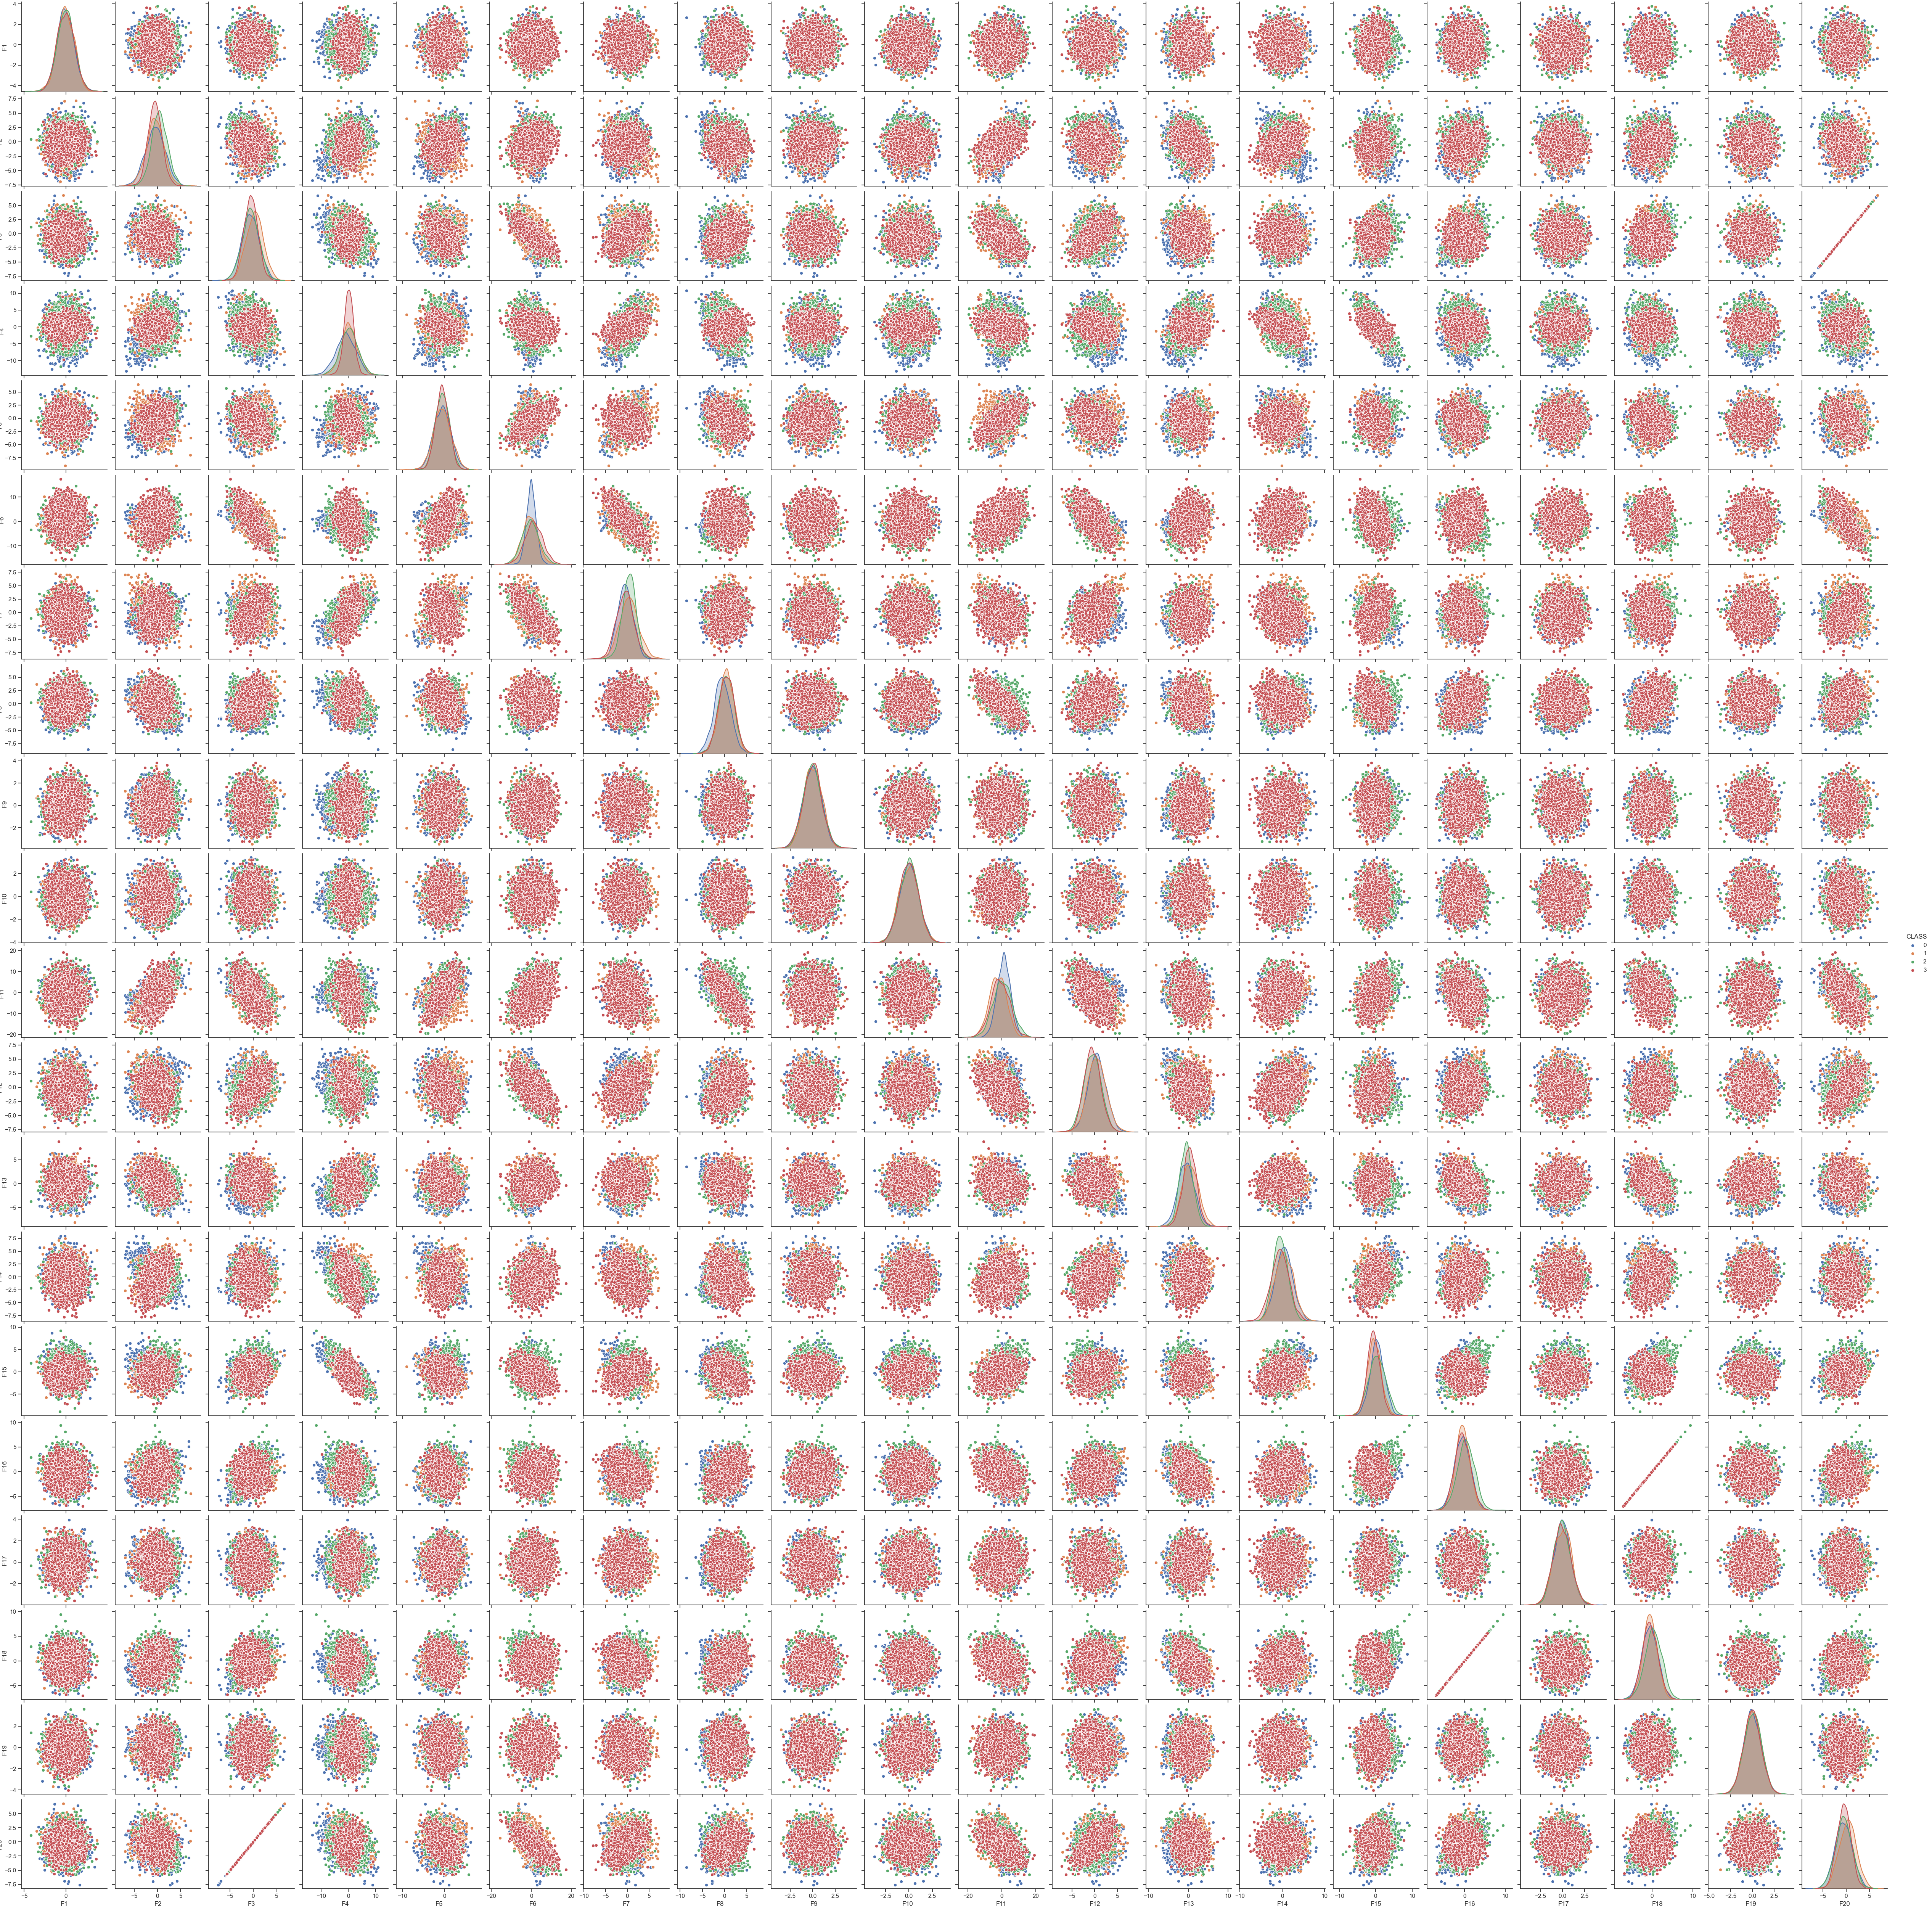
\includegraphics[width=175mm]{training_set}
                            \caption{Pair plot representing \textit{features}.}
                            \label{fig:training_set_pairplot}
                        \end{figure}
                        \clearpage
                
                \subsubsection{Data sampling} 
                
                        Il \textit{dataset} considerato presenta elementi così distribuiti:
                        \begin{itemize}
                                \item \textit{Class 1}: $33.67 \, \%$
                                \item \textit{Class 2}: $15.99 \, \%$
                                \item \textit{Class 3}: $20.66 \, \%$
                                \item \textit{Class 4}: $29.68 \, \%$
                        \end{itemize}
                        
                        \`E stato quindi effettuato balancing delle classi per evitare che il modello finale pecchi nel riconoscimento di classi meno presenti nel \textit{training set}.
                        
                        La tecnica di balancing utilizzata è lo \textit{SMOTE}.
                

        \subsection{Hyper-parameters tuning}
        
                I modelli utilizzati per la classificazione sono:
                \begin{itemize}
                        \item \textit{Multi-Layer Perceptron}
                        \item \textit{Support Vector Machine}
                        \item \textit{Decition Tree}
                        \item \textit{Random Forest}
                        \item \textit{K-Nearest Neighbors}
                        \item \textit{Stochastic Gradient Descent}
                        \item \textit{Ada Boost}
                        \item \textit{Naive Bayes}
                        \item \textit{K-Means}
                \end{itemize}
            
                In questa fase sono stati cercati gli \textit{iper-parametri} per i vari classificatori.
                

        \subsection{Evaluation}
        
                I modelli di \textit{machine learning} analizzati sono stati valutati utilizzando \textit{f1-score}.
                
                \textbf{TODO - scrivere formule f1-score ecc.}
                \bigbreak